\documentclass[a4paper, 11pt]{article}

\usepackage[absolute]{textpos} % absolute positioned text blocks
\setlength{\TPHorizModule}{1mm}
\setlength{\TPVertModule}{1mm}
\usepackage[english]{babel}
\usepackage{csquotes}

% Images
\usepackage{graphicx,wrapfig} % used for images
\graphicspath{ {./img/} }
\usepackage[labelfont=bf]{caption}

% Formatting
\usepackage{geometry} % better margins for document
\usepackage{titlesec} % better control over title spacing 
\usepackage{tabularx} % better tables
\usepackage[hidelinks]{hyperref} % hrefs
\usepackage{totcount}
\usepackage{pgfplots}
\pgfplotsset{compat=1.16}
\pgfplotsset{
    colormap={cool}{rgb255(0cm)=(237,66,76); rgb255(0.5cm)=(255,255,255); rgb255(1cm)=(57,146,239)}
}
\usepgfplotslibrary{colorbrewer}

\usepackage{float} % image placement
\usepackage{amssymb} % math symbols

% Code listings
\usepackage{listings}
\usepackage{commath}
\usepackage{pifont}
\usepackage[misc,weather,alpine]{ifsym}
\usepackage{xcolor}
\definecolor{codered}{rgb}{0.93,0.26,0.298}
\definecolor{codegrey}{rgb}{0.65,0.65,0.65}
\definecolor{codepink}{rgb}{0.737,0.47,0.823}
\definecolor{codeblue}{rgb}{0.227,0.572,0.937}
\definecolor{codegreen}{rgb}{0.441,0.664,0.286}
\definecolor{codestring}{rgb}{0.58,0,0.82}
\definecolor{backcolor}{rgb}{0.95,0.95,0.95}
\definecolor{lightgrey}{rgb}{0.8,0.8,0.8}
\definecolor{darkcyan}{RGB}{0,115,192}
\definecolor{darkercyan}{RGB}{75,101,126}
\definecolor{darkdarkcyan}{RGB}{0,65,95}

\lstdefinelanguage{HLSL}{
	morekeywords=[1]{
        % variables
        i,j,x,y,z,r,g,b,a,frequency,amplitude,current,total,maxValue,
        data,renderer,d1,d2,d3,
        baseCell,cell,seed,dMin,d,p,co,period,tiledCell,
        _Result,_NoiseScale,id,_NoiseTexture3D,
        threadCoord,noiseCoord,samplePos,noise,detail0,detail1,detail2,color,
        worldPos
	},
	morekeywords=[2]{
        % methods and functions
        vert,frag,
		distance,normalize,min,max,dot,pow,sin,cos,tan,fract,length,smoothstep,
        random2d,random,random3d,randomSeed,floor,fbm,
        random3dTo3d,random3dTo1d,tex3D,tex2D,
        renderClouds,mod,sampleDensity,
        voronoi,
        CSMain,CSNoise,numthreads
	},
	morekeywords=[3]{
        % CONSTANTS
        STEP_SIZE,MAX_STEPS,MINIMUM_STEP_SIZE,SURFACE_DISTANCE,MAX_DISTANCE,EPSILON,
        AO_ITERATIONS,AO_INTENSITY,AO_STEP_SIZE,
        LACUNARITY,GAIN,OCTAVES,TODAY,
        SV_DispatchThreadID,
        SV_Target,TEXCOORD0,TEXCOORD1,TEXCOORD2,SV_POSITION,POSITION
    },
	% morekeywords=[4]{
    %     % Unity Variables
    %     _VoronoiScale,_VoronoiOffset,,_VoronoiOctaves,_VoronoiPersistance,_VoronoiDensityThreshold,_VoronoiDensityMultiplier,
    %     _PerlinScale,_PerlinOffset,_PerlinOctaves,_PerlinPersistance,_PerlinDensityThreshold,_PerlinDensityMultiplier,
    % },
    keywordstyle=[1]\color{codeblue},
    keywordstyle=[2]\color{codered},
    keywordstyle=[3]\color{codepink},
    % keywordstyle=[4]\color{codegreen},
	commentstyle=\color{codegrey},
	morestring=[b]", % defines that strings are enclosed in double quotes
	morestring=[b]', % defines that strings are enclosed in single quotes
    backgroundcolor=\color{backcolor},
    stringstyle=\color{codered},
    numberstyle=\tiny,
    basicstyle=\ttfamily\footnotesize,
    breakatwhitespace=false,
    breaklines=true,
    captionpos=b,
    keepspaces=true,
    numbers=left,
    numbersep=5pt,
    showspaces=false,
    showstringspaces=false,
    showtabs=false,
	tabsize=2,
    sensitive=false, % keywords are not case-sensitive
    morecomment=[l]{//}, % l is for line comment
    morecomment=[s]{/*}{*/}, % s is for start and end delimiter
    belowskip=2em,
    aboveskip=1em,
}

% Gantt charts
\usepackage{pgfgantt}

% drawings
\usepackage{svg}
\usepackage{tikz}
\usepackage{fontawesome}
\usetikzlibrary{positioning, shapes}
\usetikzlibrary{arrows.meta}
\usetikzlibrary{svg.path}
\geometry{
	a4paper,
	left=28mm,
	right=28mm,
    top=30mm,
    bottom=30mm
}

% Colors 
\RequirePackage{color}
\definecolor{bfhgrey}{rgb}{0.41,0.49,0.57}
\definecolor{brinkpink}{rgb}{1.0, 0.65, 0.79}
\definecolor{columbiablue}{rgb}{0.61, 0.87, 1.0}

% Glossary
\usepackage[toc]{glossaries}
% Acronyms
\newglossaryentry{hlsl}{name={HLSL}, text={HLSL}, first={high-level shading language (HLSL)}, description={High-level shading language. Developed by microsoft, this is a standard shader language for DirectX used in graphics programming}}
\newglossaryentry{json}{name={JSON}, text={JSON}, first={Java-Script object notation (JSON)}, description={Java-Script object notation. A light-weight data format that is stored as human-readable text}}
\newglossaryentry{slpk}{name={SLPK}, text={SLPK}, first={ESRI scene layer package (SLPK)}, description={ESRI scene layer package A custom, web-optimized format used for files related to ESRI }}
\newglossaryentry{png}{name={PNG}, text={PNG}, first={portable network graphic (PNG)}, description={Portable network graphic. A common format for lossless compressed image files}}
\newglossaryentry{ui}{name={UI}, text={UI}, first={user interface (UI)}, description={User interface. The interface that allows the user to interact with the software}}
\newglossaryentry{gpu}{name={GPU}, text={GPU}, first={GPU}, description={Graphics processing unit. A piece of hardware designed to rapidly manipulate and alter memory, often intented for output to a display device}}
\newglossaryentry{wmo}{name={WMO}, text={WMO}, first={World Meteorological Organization (WMO)}, description={A specialized agency conducting atmospheric science, climatology, hydrology and geophysics}}
\newglossaryentry{rop}{name={ROP}, text={ROP}, first={render output pipeline (ROP)}, description={The render output pipeline, a component responsible for calculating the final pixel colors or depth values via specific matrix and vector operations}}
\newglossaryentry{hdrp}{name={HDRP}, text={HDRP}, first={high definition render pipeline (HDRP)}, description={Unity\'s render workflow for high fidelity, high quality projects}}
\newglossaryentry{fps}{name={FPS}, text={FPS}, first={FPS}, description={Frames per second, a measurement of how fast the application is performing (60 is good) }}

% Glossary entries
\newglossaryentry{latex}{name=LaTeX, description={ A high-quality document preparation system designed for the production of technical and scientific documentation }}
\newglossaryentry{noisegeneration}{name=Noise generation, text={noise generation}, description={ Noise generation is used to generate textures of one or more dimension with seemingly random smooth transitions from black to white (zero to one) }}
\newglossaryentry{volumetric}{name=Volumetric, text={volumetric}, description={ This describes a technique which takes a 3D volume of data and projects it to 2D. It is mostly used for transparent effects stored as a 3D image }}
\newglossaryentry{raymarching}{name=Ray marching, text={ray marching}, description={ Ray marching is a type of method to approximate the surface distance of a volumetric object, where a ray is cast into the volume and stepped forward until the surface is reached }}
\newglossaryentry{lightmarching}{name=Light marching, text={light marching}, description={ The same concept as \gls{raymarching}, but instead of being cast into the volume, it is cast towards the primary light source with a constant step }}
\newglossaryentry{billboard}{name=Billboard, text={billboard}, description={ A 2D image always facing towards the main camera }}
\newglossaryentry{worldspace}{name=World space, text={world space}, description={ Coordinates defined with respect to a global Cartesian coordinate system }}
\newglossaryentry{polymesh}{name=Polymesh, text={polymesh}, description={ A polymesh is a 3D model composed of polygons or triangles }}
\newglossaryentry{lowpoly}{name=Low poly, text={low poly}, description={ A 3D polymesh with a relatively low count of polygons }}
\newglossaryentry{scalarfield}{name=Scalar field, text={scalar field}, description={ A scalar field describes a typically three-dimensional grid of elements called \textit{voxels}, each containing a scalar value }}
\newglossaryentry{vectorfield}{name=Vector field, text={vector field}, description={ It is the same as a scalar field, except the voxels are vector values }}
\newglossaryentry{spheretracing}{name=Sphere tracing, text={sphere tracing}, description={ Sphere tracing describes an optimized algorithm of ray marching by using signed distance functions to approximate the surface distance of the volume }}
\newglossaryentry{sdf}{name=Signed distance function, text={signed distance function}, description={ A signed distance function, short SDF, returns a positive distance if the origin is outside the volume and a negative distance if it is inside the volume }}
\newglossaryentry{surfacenormal}{name=Surface normal, text={surface normal}, description={ A \textit{surface normal} or \textit{normal} is a vector which is perpendicular to a given geometry, like a triangle or polygon }}
\newglossaryentry{gradient}{name=Gradient, text={gradient}, description={ The \textit{gradient} denotes the direction of the greatest change of a scalar function }}
\newglossaryentry{penumbra}{name=Penumbra, text={penumbra}, description={ The partially shaded outer region of diffuse shadows. Also described as soft edges }}
\newglossaryentry{shapeblending}{name=Shape blending, text={shape blending}, description={ In SDFs, shapes can be seemingly blended together by returning a interpolated value of those distances }}
\newglossaryentry{ambientocclusion}{name=Ambient occlusion, text={ambient occlusion}, description={ Also known as contact shadows, this method darkens points in the scene that are not or only slightly exposed to the light and its environment }}
\newglossaryentry{noise}{name=Noise, text={noise}, description={ A randomly generated pattern, referring to \gls{procedural} pattern generation }}
\newglossaryentry{translucent}{name=Translucent, text={translucent}, description={ An object or substance that is translucent allows light to be passed through it, meaning it is rendered transparently to some degree }} 
\newglossaryentry{parameters}{name=Parameters, text={parameters}, description={ Shader variables exposed to the Unity Editor }} 
\newglossaryentry{sss}{name=Subsurface scattering, text={subsurface scattering}, description={ SSS is a mechanism of light transport in which light enters a translucent object, is scattered around and exits the material at a different point, resulting in illuminated areas where the material is thin }} 
\newglossaryentry{sunlightforwarding}{name=Sunlight forward scattering, text={sunlight forward scattering}, description={ The process of sunlight shining through and illuminating the clouds which cover the sun }} 
\newglossaryentry{sunlighttransmittance}{name=Sunlight transmittance, text={sunlight transmittance}, description={ In this matter, the same as \gls{sunlightforwarding} }} 
\newglossaryentry{cnn}{name=Convolutional neural network, text={convolutional neural network}, description={ A \gls{neuralnetwork} that is able to classify images }} 
\newglossaryentry{gan}{name=Generative adverserial network, text={generative adverserial network}, description={ A set of two \gls{neuralnetwork}s, where one generates images and the other tries to tell wether those images are real or generated }} 
\newglossaryentry{aabb}{name=Axis-aligned bounding box, text={axis-aligned bounding box}, description={ A non-rotated bounding box enclosing an object completely }} 
\newglossaryentry{shader}{name=Shader, text={shader}, description={ A piece of software which runs on the \gls{gpu}, rendering geometrically defined objects to the screen  }} 
\newglossaryentry{computeshader}{name=Compute shader, text={compute shader}, description={ A shader which runs on the GPU but outside of the default render pipeline }} 
\newglossaryentry{fbm}{name=Fractal Brownian motion, text={fractal Brownian motion}, description={ Different iterations of continuously more detailed noise layered on top of each other }} 
\newglossaryentry{fractalnoise}{name=Fractal noise, text={fractal noise}, description={ In this matter, the same as \gls{fbm} }} 
\newglossaryentry{procedural}{name=Procedural, text={procedural}, description={ Created solely with algorithms and independant of any prerequisites }}
\newglossaryentry{histogram}{name=Histogram, text={histogram}, description={ A graphical representation of data like brightness or color distribution of a given photograph }}
\newglossaryentry{csg}{name=Constructive solid geometry, text={constructive solid geometry}, description={ Short CSG, stands for combining primitive geometric objects with Boolean operators }}
\newglossaryentry{neuralnetwork}{name=Neural network, text={neural network}, description={ A series of algorithms that can recognize and categorize certain patterns in a given set of data }}
\newglossaryentry{interpolation}{name=Interpolation, text={interpolation}, description={ In mathematics, interpolation describes a method of estimating unknown values that fall between known values }}
\newglossaryentry{wrs}{name=Weather rendering system, text={weather rendering system}, description={ The Unity application that is implemented during this project. It takes in live data from a weather service and uses topological elevation models to create a weather simulation, which is then rendered and up for comparison with live photographs }}
\newglossaryentry{altitude}{name=Altitude, text={altitude}, description={ A vertical distance measurement, in this context specifically the distance from sea level to the given object }}
\newglossaryentry{watervapor}{name=Water vapor, text={water vapor}, description={ Evaporated water in a gaseous form }}
\newglossaryentry{desublimation}{name=Desublimation, text={desublimation}, description={ The process of gas transitioning to liquid without passing through the liquid phase }}
\newglossaryentry{halophenomenon}{name=Halo phenomenon, text={halo phenomenon}, description={ White or colored rings or arcs of light around the sun or the moon, produced by cirrostratus clouds }}
\newglossaryentry{cloudlet}{name=Cloudlet, text={cloudlet}, description={ Small, white, puffy clouds that come in large quantities, together forming a cloud of the cumulus family }}
\newglossaryentry{precipitation}{name=Precipitation, text={precipitation}, description={ Rainfall. The result of atmospheric water vapor that has been condensed and now falls from clouds }}
\newglossaryentry{convection}{name=Convection, text={convection}, description={ The process of warm air rising from the surface and cooling at higher altitude, of which the moisture is then condensed into clouds }}
\newglossaryentry{thermal}{name=Thermal, text={thermal}, description={ In relation with meteorology, the hot, rising air from convection is called "thermal" }}
\newglossaryentry{weatherfront}{name=Weather front, text={weather front}, description={ A boundary between to air masses, which differ in temperature, wind direction and humidity }}
\newglossaryentry{warmfront}{name=Warm front, text={warm front}, description={ A warm \gls{weatherfront}, the boundary of a mass of air that carries mild or warm air. When colliding with a \gls{coldfront}, \gls{precipitation} is often followed }}
\newglossaryentry{coldfront}{name=Cold front, text={cold front}, description={ A cold \gls{weatherfront}, the boundary of a mass of air that carries cold or cool air. When colliding with a \gls{warmfront}, \gls{precipitation} is often followed }}
\newglossaryentry{occludedfront}{name=Occluded front, text={occluded front}, description={ When a cold front overtakes a warm front, it pushes the warm air upwards (\gls{thermal}s). The moisture of the warm air condenses as it rises, creating \gls{watervapor}. This often results in clouds with \gls{precipitation} }}
\newglossaryentry{occlusion}{name=Occlusion, text={occlusion}, description={ In meteorology, the clash of a warm front and a cold front. See \gls{occludedfront} }}
\newglossaryentry{lerp}{name=Linear interpolation, text={linear interpolation}, description={ Simply put, linear interpolation describes a method of finding values inbetween two points on the same line }}
\newglossaryentry{particlesystem}{name=Particle system, text={particle system}, description={ In computer graphics, a particle system is a technique that continuously spawns and recycles objects. They are often used to reproduce fire or smoke effects, with small flame or dust textures as particles }}
\newglossaryentry{pseudorandom}{name=Pseudo-random, text={pseudo-random}, description={ A random number generated with a deterministic algorithm, meaning that the same input will always give the same output }}
\newglossaryentry{textureslice}{name=Texture slice, text={texture slice}, description={ A 2D texture extracted from a 3D texture for a given depth }}
\newglossaryentry{framebuffer}{name=Frame buffer, text={frame buffer}, description={ The buffer that stores pixels for each frame, from which the monitor constantly reads. The monitor then displays those pixels on the screen }}
\newglossaryentry{kernel}{name=Kernel, text={kernel}, description={ In \gls{computeshader}s, the kernel represents an entry point and defines the method that is executed for each thread group when running the \gls{computeshader} }}
\newglossaryentry{texel}{name=Texel, text={texel}, description={ Short for texture element, a single pixel of a 2D texture }}
\newglossaryentry{voxel}{name=Voxel, text={voxel}, description={ Short for volume element, a single element of a 3D array or 3D texture }}
\newglossaryentry{fragment}{name=Fragment, text={fragment}, description={ In computer graphics, a fragment is a single pixel on the screen that is processed by a \gls{fragmentshader} and given a color in the process, effectively rendering it }}
\newglossaryentry{fragmentshader}{name=Fragment shader, text={fragment shader}, description={ A \gls{shader} that processes single pixels, called \gls{fragment}s, calculates its color and outputs that to the \gls{framebuffer} }}
\newglossaryentry{rasterization}{name=Rasterization, text={rasterization}, description={ Rasterization describes the final step in rendering. It is the task of taking an image described in vector geometry and converting it into a raster image (a series of pixels) }}
\newglossaryentry{framerate}{name=Frame rate, text={frame rate}, description={ The rate at which a new image (called frame) appears on the display }}
\newglossaryentry{shadowpass}{name=Shadow pass, text={shadow pass}, description={ A second \gls{shader} pass that only calculates the shadow of its object }}
\newglossaryentry{proxyobject}{name=Proxy object, text={proxy object}, description={ Regarding this project, proxy objects are game objects that substitute a certain visual effect like the halo of the sun or the darkening of the sky }}
\newglossaryentry{proxyplane}{name=Proxy plane, text={proxy plane}, description={ A \gls{proxyobject} that is a plane }}
\newglossaryentry{pp}{name=Post-processing, text={post-processing}, description={ The act of applying additional effects to a rendered image before displaying it on the monitor }}
\newglossaryentry{updateloop}{name=Update loop, text={update loop}, description={ The process that updates all components every frame, like updating the scene view and game objects }}
\newglossaryentry{inengine}{name=In-engine, text={in-engine}, description={ In computer graphics, this refers to being inside the game engine; being measured or rendered by the game engine }}
\makenoidxglossaries

\glsunset{gpu}

% Bibliography
\usepackage[backend=biber, style=ieee]{biblatex}
\addbibresource{partials/paper.bib}

% add another lavel of headings
%\setcounter{tocdepth}{4}
\setcounter{secnumdepth}{4}
\titleformat{\paragraph}
{\normalfont\normalsize\bfseries}{\theparagraph}{1em}{}
\titlespacing*{\paragraph}
{0pt}{3.25ex plus 1ex minus .2ex}{1.5ex plus .2ex}

\begin{document}

\color{black}

\title{\doctitle}
\author{\docauthor}
\date{\versiondate}

\newcounter{requirements}
\newtotcounter{versionnumber}
\newcommand{\docsubtitle}{Project documentation}
\newcommand{\docauthor}{Matthias Thomann}
\newcommand{\doctitle}{Real-time Weather Rendering System}
\newcommand{\fieldofstudies}{BSc in Computer Science}
\newcommand{\specialisation}{Computer perception and virtual reality}
\newcommand{\prof}{Prof. Urs K\"unzler}

\newcommand{\versiondate}{\today}
\newcommand{\sectionref}[1]{\autoref{#1}}
\newcommand{\emptyline}{\vspace{\baselineskip}\\\noindent}

\titlespacing*{\section} {0pt}{7.5ex plus 1ex minus .2ex}{2.3ex plus .2ex}
\titlespacing*{\subsection} {0pt}{4.25ex plus 1ex minus .2ex}{1.5ex plus .2ex}

\pagenumbering{roman}
\setcounter{page}{3}

\input{partials/title.tex}
\clearpage

\section*{Abstract}
Clouds contribute a substantial part to the overall ambience in games, but an implementation of such effects often proves to be more challenging than anticipated.
To get as close as possible to real clouds, this project engages in researching and developing a near real-time weather rendering system.
This means that real weather forecasts from \emph{meteoblue} are used to visualize past, current and future weather at any given time of day.
The environment is created with elevation model data from \emph{ArcGIS}. Live photographs from \emph{Roundshot} cameras can be viewed side-by-side with the rendered output.
\\
The document dives into the science of clouds and illustrates the ten distinct classifications and how each of those could be represented in a weather simulation. 
In order to achieve high fidelity, the implementation relies on concepts like Voronoi \gls{noisegeneration} and \gls{raymarching}, which means to generate a random 3D cloud pattern and render it in volumetrically.
\\
At last, the goal of the project is to create a fully featured, near real-time weather rendering system in Unity.
It is able to render \gls{procedural} and volumetric cloudscapes, for any given date and time.
An intuitive user interface allows the user to control the weather simulation manually or let it run automatically based on \emph{meteoblue} weather reports.
\\
For future work, the weather rendering system could be incorporated in a game or further improved to achieve even higher visual realism.
\clearpage

\tableofcontents
\clearpage

\pagenumbering{arabic}

\section{General}

\subsection{Purpose}
This document serves the purpose of defining and clarifying the goals, which the thesis 'Realtime Weather Rendering System' is supposed to achieve. Furthermore, the requirement specification allows for a more accurate evaluation of the achievement of objectives and of the result itself.

\subsection{Revision History}
\begin{tabularx}{\textwidth}{|c|c|c|X|}
    \hline
    \textbf{Version}         & \textbf{Date}        & \textbf{Name}     & \textbf{Comment}                  \\ \hline \addtocounter{versionnumber}{1}
    0.\arabic{versionnumber} & February 27, 2021    & Matthias Thomann  & Initial draft                     \\ \hline
\end{tabularx}
\clearpage
\section{Natural Clouds}
Clouds are a substantial part of Earth's weather. They provide shade from the glistening sun on hot days and reflect the heat at night, keeping the ground warmer.
For a layman, clouds are comprehensible and useful indicators for telling the weather. If they are dark and low-hanging, they bring rain. If they are puffy and scarce, they predict fair weather ahead.

\subsection{Types of Clouds}
In order to create a \gls{wrs} that is able to display many different cloudscapes, all distinct types of clouds have to be understood first.
Natural clouds are typically identified by two major factors: shape and \gls{altitude}.

\begin{figure}[H]
    \includegraphics[width=\linewidth]{clouds-types.jpg}
    \captionof{figure}{Different categorizations of cloudshapes \protect\cite{cloudtypes}.}
    \label{img:ui:mockup:live}
\end{figure}

\noindent
This graphic from \emph{sciencelearn} provides and excellent overview of all distinct cloud types.
Each type is depicted in its signature shape and marked with the scientific name and abbreviation.

% refs:
% https://www.countryfile.com/how-to/outdoor-skills/how-to-predict-the-weather-forecast-using-clouds/
% NASA how do clouds form: https://climatekids.nasa.gov/cloud-formation/#:~:text=Clouds%20are%20created%20when%20water,are%20floating%20in%20the%20air.&text=That%20means%20some%20of%20the,drifted%20away%20into%20the%20atmosphere.
% NASA: https://www.nasa.gov/audience/forstudents/k-4/stories/nasa-knows/what-are-clouds-k4.html


\subsubsection{Classification of Altitude}
The \gls{altitude}, which is the distance from sea level to the cloud, is further split into three categories "low", "mid" and "high". 

\subsubsection{Classification of Shape}
\clearpage
\section{Implementation Approach}
Clouds are comprehensible indicators for telling the weather. 
They offer many visible features to make an rough prediction of the weather conditions, or weather changes to come.
As described in \sectionref{section:clouds:types}, some cloud types only form under specific conditions.
Also, whenever certain clouds are present, \gls{precipitation} is shortly followed, as it is with altostratus clouds.
\\
Those factors allow a prediction of the weather, but for this project, the process is reversed.
The given data is not an image of clouds, but meteorological measurement data, and the desired outcome is not a prediction, but an image of clouds.

\begin{figure}[H]
    \centering
    \begin{minipage}{0.47\linewidth}
        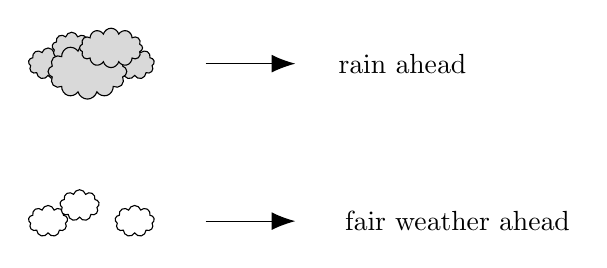
\begin{tikzpicture}
            \tikzset{edge/.style = {-{Latex[length=3mm]},shorten >= -4pt}}
            \tikzset{shortedge/.style = {shorten <=-4pt,shorten >= -4pt}}
            \tikzset{shortshortedge/.style = {shorten <=-5.5pt,shorten >= -5.3pt}}
            \tikzset{shortshortedge2/.style = {shorten <=-4.5pt,shorten >= -4.5pt}}

            % rainy clouds
            \node (cloud1) at (0.5, 2.0) {};
            \node (cloud2) at (0.8, 2.2) {};
            \node (cloud5) at (1.6, 2.0) {};
            \node (cloud3) at (1.0, 1.9) {};
            \node (cloud4) at (1.3, 2.2) {};
            \node[cloud,fill=gray!30,cloud puffs=9, cloud, minimum width=0.5cm, minimum height=0.2cm, align=center, draw] (cloud) at (cloud1) {};
            \node[cloud,fill=gray!30,cloud puffs=9, cloud, minimum width=0.5cm, minimum height=0.2cm, align=center, draw] (cloud) at (cloud2) {};
            \node[cloud,fill=gray!30,cloud puffs=9, cloud, minimum width=0.5cm, minimum height=0.2cm, align=center, draw] (cloud) at (cloud5) {};
            \node[cloud,fill=gray!30,cloud puffs=12, cloud, minimum width=1.0cm, minimum height=0.7cm, align=center, draw] (cloud) at (cloud3) {};
            \node[cloud,fill=gray!30,cloud puffs=12, cloud, minimum width=0.8cm, minimum height=0.5cm, align=center, draw] (cloud) at (cloud4) {};
            \draw[edge] (2.5, 2) -- (3.5,2);
            \node at (5,2) {rain ahead};

            % clear clouds
            \node (cloud1) at (0.5, 0.0) {};
            \node (cloud2) at (0.9, 0.2) {};
            \node (cloud5) at (1.6, 0.0) {};
            \node[cloud,fill=white,cloud puffs=9, cloud, minimum width=0.5cm, minimum height=0.2cm, align=center, draw] (cloud) at (cloud1) {};
            \node[cloud,fill=white,cloud puffs=9, cloud, minimum width=0.5cm, minimum height=0.2cm, align=center, draw] (cloud) at (cloud2) {};
            \node[cloud,fill=white,cloud puffs=9, cloud, minimum width=0.5cm, minimum height=0.2cm, align=center, draw] (cloud) at (cloud5) {};
            \draw[edge] (2.5, 0) -- (3.5,0);
            \node at (5.7,0) {fair weather ahead};

        \end{tikzpicture}
        \captionof{figure}{Weather information based on visual data.}
        \label{img:tikz:impl:data1}
    \end{minipage}        
    \hfill
    \begin{minipage}{0.47\linewidth}
        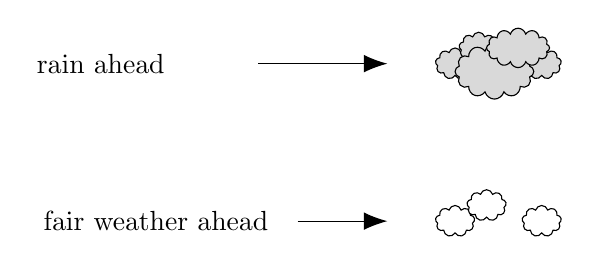
\begin{tikzpicture}
            \tikzset{edge/.style = {-{Latex[length=3mm]},shorten >= -4pt}}
            \tikzset{shortedge/.style = {shorten <=-4pt,shorten >= -4pt}}
            \tikzset{shortshortedge/.style = {shorten <=-5.5pt,shorten >= -5.3pt}}
            \tikzset{shortshortedge2/.style = {shorten <=-4.5pt,shorten >= -4.5pt}}

            % rainy clouds
            \node (cloud1) at (4.5, 2.0) {};
            \node (cloud2) at (4.8, 2.2) {};
            \node (cloud5) at (5.6, 2.0) {};
            \node (cloud3) at (5.0, 1.9) {};
            \node (cloud4) at (5.3, 2.2) {};
            \node[cloud,fill=gray!30,cloud puffs=9, cloud, minimum width=0.5cm, minimum height=0.2cm, align=center, draw] (cloud) at (cloud1) {};
            \node[cloud,fill=gray!30,cloud puffs=9, cloud, minimum width=0.5cm, minimum height=0.2cm, align=center, draw] (cloud) at (cloud2) {};
            \node[cloud,fill=gray!30,cloud puffs=9, cloud, minimum width=0.5cm, minimum height=0.2cm, align=center, draw] (cloud) at (cloud5) {};
            \node[cloud,fill=gray!30,cloud puffs=12, cloud, minimum width=1.0cm, minimum height=0.7cm, align=center, draw] (cloud) at (cloud3) {};
            \node[cloud,fill=gray!30,cloud puffs=12, cloud, minimum width=0.8cm, minimum height=0.5cm, align=center, draw] (cloud) at (cloud4) {};
            \draw[edge] (2, 2) -- (3.5,2);
            \node at (0,2) {rain ahead};

            % clear clouds
            \node (cloud1) at (4.5, 0.0) {};
            \node (cloud2) at (4.9, 0.2) {};
            \node (cloud5) at (5.6, 0.0) {};
            \node[cloud,fill=white,cloud puffs=9, cloud, minimum width=0.5cm, minimum height=0.2cm, align=center, draw] (cloud) at (cloud1) {};
            \node[cloud,fill=white,cloud puffs=9, cloud, minimum width=0.5cm, minimum height=0.2cm, align=center, draw] (cloud) at (cloud2) {};
            \node[cloud,fill=white,cloud puffs=9, cloud, minimum width=0.5cm, minimum height=0.2cm, align=center, draw] (cloud) at (cloud5) {};
            \draw[edge] (2.5, 0) -- (3.5,0);
            \node at (0.7,0) {fair weather ahead};
            
        \end{tikzpicture}
        \captionof{figure}{Visual construction based on weather information.}
        \label{img:tikz:impl:data2}       
    \end{minipage}
\end{figure}

\noindent
For any given day to render, an implementation would require data from that day but also from the near future of that day.
So, in order to render a cloud image for day $x$, a potential algorithm could look like this.
Note that the listing below describes only an idea and is by no means final or compulsory.

\begin{lstlisting}[language=HLSL, caption=Pseudo-code of cloud render algorithm., label=lst:pseudo:algorithm]
// weather data including 7-day forecast
WeatherData data;

function renderClouds(Day x) {
    if (x > TODAY + 7) throw;

    d1 = data.getDataFor(x);
    d2 = data.getDataFor(x + 1);
    d3 = data.getDataFor(x + 2);
    // and so on...

    // sophisticated checks about current and future conditions:
    if (d1.fairWeather && d2.fairWeather)
        return renderer.clearSky();
    if (d1.fairWeather && d2.isRaining)
        return renderer.cloudsOnclearDayBeforeRain();
    if (d1.isRaining)
        return renderer.cloudsOnRainyDay();
    if (d2.isRaining) 
        return renderer.cloudsBeforeRainyDay();
    if (d3.isRaining) 
        return renderer.clouds2DaysBeforeRainyDay();
    // and so on...
    
}
\end{lstlisting}

\clearpage

\subsection{Look-Ahead Issue}
The approach as described above relies on having data from a couple of days ahead of time. Assumed that number of days is $t$, then the weather data for day $x$ could only be rendered $t$ days after $x$.
That would mean, for such an approach to work, the weather of today can not be rendered before $t$ days later.
\\
In this case however, the weather measurement data retrieved from \emph{meteoblue} also contains a seven-day weather forecast. 
Given that $t$ is less than or equal to seven and an implementation still produces accurate cloud imagery, it would no longer be an issue.

\subsection{Layers of Cloud Shaders}
As identified in \sectionref{section:clouds:types}, most of the clouds in the troposhpere only appear at certain \gls{altitude}s.
The high-level clouds are all of type \emph{cirrus}.
The mid-level clouds are both of type \emph{alto} and similar in look, while most of the low-level clouds belong to the \emph{cumulus} family.
\\
This leads to the conclusion that some of the cloud types could be combined into a single layer and rendered by the same shader.
Exception to that are only the two larger types that span over multiple height levels: nimbostratus and cumulonimbus. For those, a more unique solution has to be found.

\begin{figure}[H]
    \centering
    \begin{tikzpicture}[scale=1]
        \tikzset{edge/.style = {-{Latex[length=3mm]},shorten >= -4pt}}
        \tikzset{shortedge/.style = {shorten <=-4pt,shorten >= -4pt}}
        \tikzset{icon/.style = {font=\Large}}

        % icons
        \node[red,icon] (cam) at (0.1, 5.2) {\faVideoCamera};
        \node[red,yshift=-0.5cm,xshift=-0.3cm] at (cam) {camera};
        \draw (0.5,5.45) -- (2,7);
        \draw (0.5,4.95) -- (2,3.5);

        % cloud layer boxes
        \draw (3,7) rectangle (10,6.2);
        \draw (3,6) rectangle (10,5.2);
        \draw (3,5) rectangle (10,4.2);
        \draw (3,4) rectangle (10,2.2);
        \node at (6.5,6.6) {cirrus layer};
        \node at (6.5,5.6) {alto layer};
        \node at (6.5,4.6) {stratus layer};
        \node at (6.5,3.1) {fog layer};

        % houses
        \node[black!40] at (4.9, 1.15) {\faHome};
        \node[black!40] at (5.2, 1.20) {\faHome};
        \node[black!40] at (5.4, 1.24) {\faHome};
        \node[black!40,icon] at (5.7, 1.25) {\faHome};
        \node[black!40] at (6.0, 1.15) {\faHome};
        \node[black!40] at (6.35, 1.22) {\faHome};
        \node[black!40] at (6.8, 1.4) {\faUniversity};
        \node[black!40] at (7.1, 1.32) {\faHome};
        \node[black!40] at (7.5, 1.25) {\faHome};
        \node[black!40,icon] at (7.8, 1.23) {\faHome};
        \node[black!40] at (8.1, 1.16) {\faHome};
        \node[black!60] at (6.4,0.7) {city of Bern};
        
        % ground
        \node[green!50!black,rotate=-58,anchor=west] at (1.2,3.1) {ground};
        \draw[green!50!black,thick] (0,4.2) -- (0.2,4.2) -- (0.4,4.1) -- (0.5,4) -- (1,3) -- (2,1.5) -- (3,1.1) -- (5,1) -- (5.1,1.05) -- (5.4,1.1) -- (6,1) -- (6.5,1.1) -- (6.6,1.2) -- (7,1.2) -- (8,1) -- (10,1.1);

        % height of troposphere
        \draw (12.0,1) -- (12.0,7);
        \draw (12.1,1) -- (11.9,1);
        \draw (12.1,7) -- (11.9,7);
        \node[rotate=90,anchor=west] at (11.7,2.5) {troposphere height};

    \end{tikzpicture}
    \captionof{figure}{Shader setup.}
    \label{img:tikz:shadersetup}       
\end{figure}

\subsubsection{Cirrus Layer}
The uppermost layer would contain cirrus, cirrostratus and cirrocumulus clouds.
All of these form under similar weather conditions and closely resemble each other in appearance.
\\
A potential \gls{shader} could be programmed to render either no clouds at all or a base variant of all three cirrus clouds, which could then be parametrized into an individual type of cirrus cloud.

\begin{figure}[H]
    \includegraphics[width=\linewidth]{cloudlayers/cirruslayer.png}
    \caption{A breakdown of the cirrus cloud layer.}
    \label{img:cloudlayer:cirrus}
\end{figure}

\subsubsection{Alto Layer}
The middle layer consists of altostratus and altocumulus clouds, the latter mainly being formed by dissipation of the former one.
Since they have many shared characteristics, apart from the puffiness, they are predestined to be combined.
\\
Given a \gls{shader} is flexible enough to render altostratus clouds, then it is also able to render altocumulus, with only few adjustements necessary.

\begin{figure}[H]
    \includegraphics[width=\linewidth]{cloudlayers/altolayer.png}
    \caption{A breakdown of the alto cloud layer.}
    \label{img:cloudlayer:alto}
\end{figure}
\clearpage
\section{Noise Generation}
\label{section:noise}
Nature's chaotic and fortuitous behavior creates a world full of diversity and unpredictability.
This can be observed in a surprisingly high amount of objects, structures and phenomenons.
\\
For example, the following images show photographs of patterns that seem almost completely random.

\begin{figure}[H]
    \includegraphics[width=\linewidth]{nature-random.png}
    \caption{Random pattern observed in Nature \protect\cite{bookofshaders:noise}.}
    \label{img:rnd:natural}
\end{figure}

\noindent
In computer science, the virtual recreation of such randomness has been studied continuously over the last decades.
The outcome of a randomness generator is called \emph{\gls{noise}}.
There are many established algorithms to create random patterns, one of which generates the famous \emph{Voronoi} \gls{noise}.

\subsection{Previous Work}
Many of the following subsections rely on concepts and algorithms that have been thorougly explained in the project's previous work \cite{project2:noise}.
This include sine-based deterministic number generation algorithms, also known as also \emph{\gls{pseudorandom}} number generation \cite{project2:noise:pseudo}.
It further includes different \gls{noisegeneration} algorithms like Perlin \gls{noise} \cite{project2:noise:perlin}.
\emptyline
Those algorithms will not be described again, as they have already been studied and documented before.

\pagebreak

\subsection{Voronoi Noise Algorithm}
\label{section:noise:voronoi}
One of the more commonly used procedural pattern generation algorithms is that of Steven Worley, developed in 1996 \cite{worley}, called \emph{Worley}'s algorithm.
The algorithm is also known as the \emph{Voronoi} algorithm due to its similar appearance to a Voronoi diagram.
In that diagram, points, called \emph{seeds}, are randomly scattered inside a defined space.
After that, regions are created, consisting of all points closer to that seed than to any other.
\\
The Voronoi \gls{noise} algorithm creates a cellular pattern and is therefore well suited for simulating natural distribution of cloud heaps, as they are in some way also arranged in cells.
\emptyline
The \gls{noise} algorithm starts by dividing the space into a grid, for which each cell is assigned a random point.
From there, each fragment gets shaded by how far it is to the seed in its cell.

\begin{figure}[H]
    \centering

    \begin{minipage}{0.47\linewidth}
        \centering
        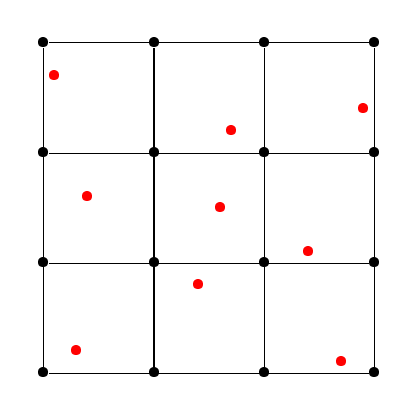
\begin{tikzpicture}[scale=0.7, x=2cm,y=2cm]
        \tikzset{c/.style = {shorten <=-4pt, shorten >=-4pt}}
        \tikzset{smalledge/.style = {-{Latex[length=2mm]},shorten <=-4pt}}
        
        \node (x1y1) at (0,0) {\textbullet};
        \node (x2y1) at (1,0) {\textbullet};
        \node (x3y1) at (2,0) {\textbullet};
        \node (x4y1) at (3,0) {\textbullet};

        \node (x1y2) at (0,1) {\textbullet};
        \node (x2y2) at (1,1) {\textbullet};
        \node (x3y2) at (2,1) {\textbullet};
        \node (x4y2) at (3,1) {\textbullet};

        \node (x1y3) at (0,2) {\textbullet};
        \node (x2y3) at (1,2) {\textbullet};
        \node (x3y3) at (2,2) {\textbullet};
        \node (x4y3) at (3,2) {\textbullet};

        \node (x1y4) at (0,3) {\textbullet};
        \node (x2y4) at (1,3) {\textbullet};
        \node (x3y4) at (2,3) {\textbullet};
        \node (x4y4) at (3,3) {\textbullet};

        \draw[c] (x1y1) edge node{} (x4y1);
        \draw[c] (x1y2) edge node{} (x4y2);
        \draw[c] (x1y3) edge node{} (x4y3);
        \draw[c] (x1y4) edge node{} (x4y4);

        \draw[c] (x1y1) edge node{} (x1y4);
        \draw[c] (x2y1) edge node{} (x2y4);
        \draw[c] (x3y1) edge node{} (x3y4);
        \draw[c] (x4y1) edge node{} (x4y4);

        \node[red] (s1) at (0.3,0.2) {\textbullet};
        \node[red] (s2) at (1.4,0.8) {\textbullet};
        \node[red] (s3) at (2.7,0.1) {\textbullet};
        \node[red] (s4) at (0.4,1.6) {\textbullet};
        \node[red] (s5) at (1.6,1.5) {\textbullet};
        \node[red] (s6) at (2.4,1.1) {\textbullet};
        \node[red] (s7) at (0.1,2.7) {\textbullet};
        \node[red] (s8) at (1.7,2.2) {\textbullet};
        \node[red] (s9) at (2.9,2.4) {\textbullet};

        \end{tikzpicture}
        \captionof{figure}{Voronoi grid with \gls{pseudorandom}ly assigned seed points for each cell.}
        \label{img:tikz:noise:voronoi}
    \end{minipage}
    \hfill
    \begin{minipage}{0.47\linewidth}
        \centering
        \begin{tikzpicture}[scale=0.7, x=2cm,y=2cm]
            \tikzset{c/.style = {shorten <=-4pt, shorten >=-4pt}}
            \tikzset{smalledge/.style = {-{Latex[length=2mm]},shorten <=-4pt}}
            
            \node (gradient) at (1.5,1.5) {\includegraphics[width=4.2cm] {noise/2d voronoi unmixed}};

            \node (x1y1) at (0,0) {\textbullet};
            \node (x2y1) at (1,0) {\textbullet};
            \node (x3y1) at (2,0) {\textbullet};
            \node (x4y1) at (3,0) {\textbullet};

            \node (x1y2) at (0,1) {\textbullet};
            \node (x2y2) at (1,1) {\textbullet};
            \node (x3y2) at (2,1) {\textbullet};
            \node (x4y2) at (3,1) {\textbullet};

            \node (x1y3) at (0,2) {\textbullet};
            \node (x2y3) at (1,2) {\textbullet};
            \node (x3y3) at (2,2) {\textbullet};
            \node (x4y3) at (3,2) {\textbullet};

            \node (x1y4) at (0,3) {\textbullet};
            \node (x2y4) at (1,3) {\textbullet};
            \node (x3y4) at (2,3) {\textbullet};
            \node (x4y4) at (3,3) {\textbullet};

            \draw[c] (x1y1) edge node{} (x4y1);
            \draw[c] (x1y2) edge node{} (x4y2);
            \draw[c] (x1y3) edge node{} (x4y3);
            \draw[c] (x1y4) edge node{} (x4y4);

            \draw[c] (x1y1) edge node{} (x1y4);
            \draw[c] (x2y1) edge node{} (x2y4);
            \draw[c] (x3y1) edge node{} (x3y4);
            \draw[c] (x4y1) edge node{} (x4y4);

            \node[red] (s1) at (0.3,0.2) {\textbullet};
            \node[red] (s2) at (1.4,0.8) {\textbullet};
            \node[red] (s3) at (2.7,0.1) {\textbullet};
            \node[red] (s4) at (0.4,1.6) {\textbullet};
            \node[red] (s5) at (1.6,1.5) {\textbullet};
            \node[red] (s6) at (2.4,1.1) {\textbullet};
            \node[red] (s7) at (0.1,2.7) {\textbullet};
            \node[red] (s8) at (1.7,2.2) {\textbullet};
            \node[red] (s9) at (2.9,2.4) {\textbullet};

        \end{tikzpicture}
        \captionof{figure}{Voronoi grid with seed distances visualized.}
        \label{img:tikz:noise:voronoi2}
    \end{minipage}
\end{figure}

\noindent
As reckognizable in \autoref{img:tikz:noise:voronoi2}, hard contours are still visible along the grid lines. This can be improved by including the adjacent cells when finding the closest seed for any given fragment.
This amounts to $3^n - 1$ neighboring cells, where $n$ is the number of dimensions. This means for 2D space its eight cells, while in 3D its 26.

\begin{figure}[H]
    \centering
    \begin{tikzpicture}[scale=1.2, x=2cm,y=2cm]
        \tikzset{c/.style = {shorten <=-4pt, shorten >=-4pt}}
        \tikzset{smalledge/.style = {-{Latex[length=2mm]},shorten <=-4pt}}
        
        \node (gradient) at (1.5,1.5) {\includegraphics[width=7.2cm] {noise/2d voronoi}};

        \node (x1y1) at (0,0) {\textbullet};
        \node (x2y1) at (1,0) {\textbullet};
        \node (x3y1) at (2,0) {\textbullet};
        \node (x4y1) at (3,0) {\textbullet};

        \node (x1y2) at (0,1) {\textbullet};
        \node (x2y2) at (1,1) {\textbullet};
        \node (x3y2) at (2,1) {\textbullet};
        \node (x4y2) at (3,1) {\textbullet};

        \node (x1y3) at (0,2) {\textbullet};
        \node (x2y3) at (1,2) {\textbullet};
        \node (x3y3) at (2,2) {\textbullet};
        \node (x4y3) at (3,2) {\textbullet};

        \node (x1y4) at (0,3) {\textbullet};
        \node (x2y4) at (1,3) {\textbullet};
        \node (x3y4) at (2,3) {\textbullet};
        \node (x4y4) at (3,3) {\textbullet};

        \draw[c] (x1y1) edge node{} (x4y1);
        \draw[c] (x1y2) edge node{} (x4y2);
        \draw[c] (x1y3) edge node{} (x4y3);
        \draw[c] (x1y4) edge node{} (x4y4);

        \draw[c] (x1y1) edge node{} (x1y4);
        \draw[c] (x2y1) edge node{} (x2y4);
        \draw[c] (x3y1) edge node{} (x3y4);
        \draw[c] (x4y1) edge node{} (x4y4);

        \node[red] (s1) at (0.3,0.2) {\textbullet};
        \node[red] (s2) at (1.4,0.8) {\textbullet};
        \node[red] (s3) at (2.7,0.1) {\textbullet};
        \node[red] (s4) at (0.4,1.6) {\textbullet};
        \node[red] (s5) at (1.6,1.5) {\textbullet};
        \node[red] (s6) at (2.4,1.1) {\textbullet};
        \node[red] (s7) at (0.1,2.7) {\textbullet};
        \node[red] (s8) at (1.7,2.2) {\textbullet};
        \node[red] (s9) at (2.9,2.4) {\textbullet};

    \end{tikzpicture}
    \captionof{figure}{Complete 2D Voronoi \gls{noise} texture.}
    \label{img:tikz:noise:voronoi3}
\end{figure}

\pagebreak

\noindent
An implementation of this relatively simple algorithm could look like the following listing.
\begin{lstlisting}[language=HLSL, caption=Implementation of 2D Voronoi \gls{noise} algorithm., label=lst:shader:noise:voronoi2d]
float2 randomSeed(float2 co) {
    return float2(
        fract(sin(dot(co, float2(12.9898, 78.233))) * 43758.5453123),
        fract(sin(dot(co, float2(39.3461, 11.135))) * 14375.8545359));
}

float voronoi(float2 p) {
    float2 baseCell = floor(p);
    float dMin = 999;

    for(int x = -1; x <= 1; x++) {
        for(int y = -1; y <= 1; y++) {
            float2 cell = baseCell + float2(x, y);
            float2 seed = cell + randomSeed(cell);
            float d = distance(seed, p);
            if (d < dMin) {
                dMin = d;
            }
        }
    }
    
    return dMin;
}
\end{lstlisting}

\noindent
The 3D equivalent of the algorithm looks fairly similar.

\begin{lstlisting}[language=HLSL, caption=Implementation of 3D Voronoi \gls{noise} algorithm., label=lst:shader:noise:voronoi3d]
float3 randomSeed(float3 co) {
    return float3(
    fract(sin(dot(co, float3(12.989, 78.233, 37.719))) * 43758.5453123),
    fract(sin(dot(co, float3(39.346, 11.135, 83.155))) * 14375.8545346),
    fract(sin(dot(co, float3(73.156, 52.235, 09.151))) * 31396.2234116));
}

float voronoi(float3 p) {
    float3 baseCell = floor(p);
    float dMin = 999;

    for(int x = -1; x <= 1; x++) {
        for(int y = -1; y <= 1; y++) {
            for(int z = -1; z <= 1; z++) {
                float3 cell = baseCell + float3(x, y, z);
                float3 seed = cell + randomSeed(cell);
                float d = distance(seed, p);
                if (d < dMin) {
                    dMin = d;
                }
            }
        }
    }
    
    return dMin;
}
\end{lstlisting}

\subsection{Seamless Noise}
\label{section:noise:seamless}
In \autoref{img:tikz:noise:voronoi3}, the generated cells appear to be randomly distributed, but there is still a major flaw in the texture.
\\
As already mentioned previously, the \gls{noisegeneration} is confined to a fixed region.
This poses an issue when the desired area is larger than the defined space of the algorithm.
It is therefore not possible to tile the same texture without visible seams inbetween the tiles.

\begin{figure}[H]
    \includegraphics[width=\linewidth]{noise/voronoi seam.png}
    \caption{Tiled 3D \gls{noise} \gls{textureslice}.}
    \label{img:rnd:noise:seam}
\end{figure}

\noindent
The problem occurs when checking the neighboring cells of the current cell. For example, here are the seeds for two adjacent tiles of the same \gls{noise} texture.

\begin{figure}[H]
    \centering
    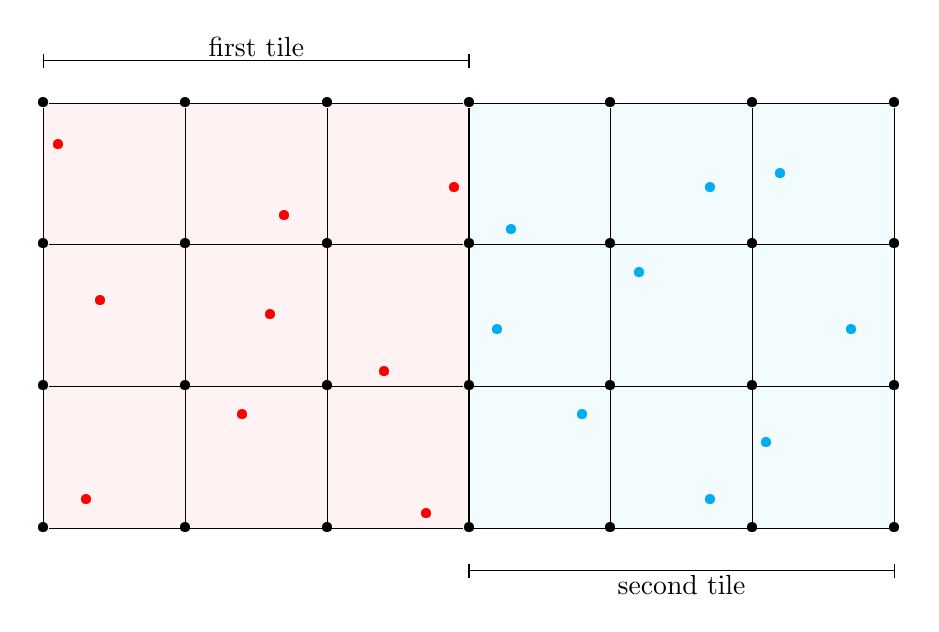
\begin{tikzpicture}[scale=0.9, x=2cm,y=2cm]
    \tikzset{c/.style = {shorten <=-4pt, shorten >=-4pt}}
    \tikzset{smalledge/.style = {-{Latex[length=2mm]},shorten <=-4pt}}
    
    % tile label 1
    \draw (0,3.3) -- (3,3.3);
    \draw (0,3.25) -- (0,3.35);
    \draw (3,3.25) -- (3,3.35);
    \node at (1.5,3.4) {first tile};
    
    % tile label 2
    \draw (3,-0.3) -- (6,-0.3);
    \draw (3,-0.25) -- (3,-0.35);
    \draw (6,-0.25) -- (6,-0.35);
    \node at (4.5,-0.4) {second tile};

    \node (offset) at (3.0,0) {};

    \fill[cyan!5] (offset) rectangle ($(offset) + (3,3)$);
    \fill[red!5] (0,0) rectangle (3,3);

    \node (x1y1) at (0,0) {\textbullet};
    \node (x2y1) at (1,0) {\textbullet};
    \node (x3y1) at (2,0) {\textbullet};
    \node (x4y1) at (3,0) {\textbullet};

    \node (x1y2) at (0,1) {\textbullet};
    \node (x2y2) at (1,1) {\textbullet};
    \node (x3y2) at (2,1) {\textbullet};
    \node (x4y2) at (3,1) {\textbullet};

    \node (x1y3) at (0,2) {\textbullet};
    \node (x2y3) at (1,2) {\textbullet};
    \node (x3y3) at (2,2) {\textbullet};
    \node (x4y3) at (3,2) {\textbullet};

    \node (x1y4) at (0,3) {\textbullet};
    \node (x2y4) at (1,3) {\textbullet};
    \node (x3y4) at (2,3) {\textbullet};
    \node (x4y4) at (3,3) {\textbullet};

    \draw[c] (x1y1) edge node{} (x4y1);
    \draw[c] (x1y2) edge node{} (x4y2);
    \draw[c] (x1y3) edge node{} (x4y3);
    \draw[c] (x1y4) edge node{} (x4y4);

    \draw[c] (x1y1) edge node{} (x1y4);
    \draw[c] (x2y1) edge node{} (x2y4);
    \draw[c] (x3y1) edge node{} (x3y4);
    \draw[c] (x4y1) edge node{} (x4y4);

    \node[red] (s1) at (0.3,0.2) {\textbullet};
    \node[red] (s2) at (1.4,0.8) {\textbullet};
    \node[red] (s3) at (2.7,0.1) {\textbullet};
    \node[red] (s4) at (0.4,1.6) {\textbullet};
    \node[red] (s5) at (1.6,1.5) {\textbullet};
    \node[red] (s6) at (2.4,1.1) {\textbullet};
    \node[red] (s7) at (0.1,2.7) {\textbullet};
    \node[red] (s8) at (1.7,2.2) {\textbullet};
    \node[red] (s9) at (2.9,2.4) {\textbullet};

    \node (x1y1) at ($(offset) + (0,0)$) {};
    \node (x2y1) at ($(offset) + (1,0)$) {\textbullet};
    \node (x3y1) at ($(offset) + (2,0)$) {\textbullet};
    \node (x4y1) at ($(offset) + (3,0)$) {\textbullet};

    \node (x1y2) at ($(offset) + (0,1)$) {};
    \node (x2y2) at ($(offset) + (1,1)$) {\textbullet};
    \node (x3y2) at ($(offset) + (2,1)$) {\textbullet};
    \node (x4y2) at ($(offset) + (3,1)$) {\textbullet};

    \node (x1y3) at ($(offset) + (0,2)$) {};
    \node (x2y3) at ($(offset) + (1,2)$) {\textbullet};
    \node (x3y3) at ($(offset) + (2,2)$) {\textbullet};
    \node (x4y3) at ($(offset) + (3,2)$) {\textbullet};

    \node (x1y4) at ($(offset) + (0,3)$) {};
    \node (x2y4) at ($(offset) + (1,3)$) {\textbullet};
    \node (x3y4) at ($(offset) + (2,3)$) {\textbullet};
    \node (x4y4) at ($(offset) + (3,3)$) {\textbullet};

    \draw[c] (x1y1) edge node{} (x4y1);
    \draw[c] (x1y2) edge node{} (x4y2);
    \draw[c] (x1y3) edge node{} (x4y3);
    \draw[c] (x1y4) edge node{} (x4y4);

    \draw[c] (x2y1) edge node{} (x2y4);
    \draw[c] (x3y1) edge node{} (x3y4);
    \draw[c] (x4y1) edge node{} (x4y4);

    \node[cyan] (s1) at ($(offset) + (0.8,0.8)$) {\textbullet};
    \node[cyan] (s2) at ($(offset) + (1.7,0.2)$) {\textbullet};
    \node[cyan] (s3) at ($(offset) + (2.1,0.6)$) {\textbullet};
    \node[cyan] (s4) at ($(offset) + (0.2,1.4)$) {\textbullet};
    \node[cyan] (s5) at ($(offset) + (1.2,1.8)$) {\textbullet};
    \node[cyan] (s6) at ($(offset) + (2.7,1.4)$) {\textbullet};
    \node[cyan] (s7) at ($(offset) + (0.3,2.1)$) {\textbullet};
    \node[cyan] (s8) at ($(offset) + (1.7,2.4)$) {\textbullet};
    \node[cyan] (s9) at ($(offset) + (2.2,2.5)$) {\textbullet};

    \end{tikzpicture}
    \captionof{figure}{Voronoi \gls{noise} seeds of the second tile are different than the seeds of the first tile.}
    \label{img:tikz:noise:seamless:1}
\end{figure}

\pagebreak

\noindent
When inspecting the cell $c_{2,1}$ of the first tile, some of its neighbors, namely $c_{3,0}$ to $c_{3,2}$, are part of the next tile.
However, since the desired outcome is a repeating texture, the next tile will be the same as the first one.

\begin{figure}[H]
    \centering
    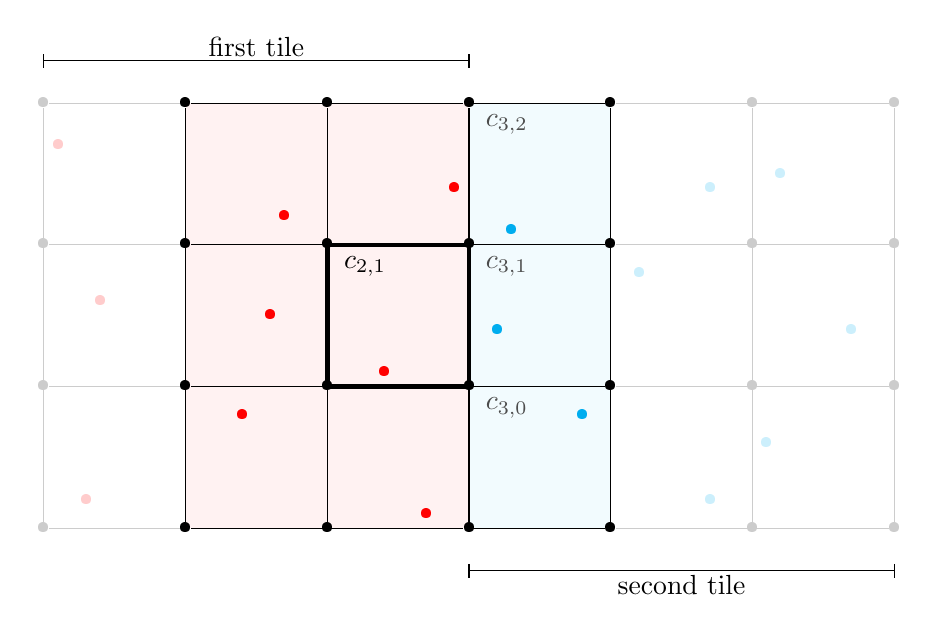
\begin{tikzpicture}[scale=0.9, x=2cm,y=2cm]
    \tikzset{c/.style = {shorten <=-4pt, shorten >=-4pt}}
    \tikzset{smalledge/.style = {-{Latex[length=2mm]},shorten <=-4pt}}
    
    % tile label 1
    \draw (0,3.3) -- (3,3.3);
    \draw (0,3.25) -- (0,3.35);
    \draw (3,3.25) -- (3,3.35);
    \node at (1.5,3.4) {first tile};
    
    % tile label 2
    \draw (3,-0.3) -- (6,-0.3);
    \draw (3,-0.25) -- (3,-0.35);
    \draw (6,-0.25) -- (6,-0.35);
    \node at (4.5,-0.4) {second tile};

    \node (offset) at (3.0,0) {};

    \fill[cyan!5] (offset) rectangle ($(offset) + (1,3)$);
    \fill[red!5] (1,0) rectangle (3,3);

    \node[black!20] (x1y1) at (0,0) {\textbullet};
    \node (x2y1) at (1,0) {\textbullet};
    \node (x3y1) at (2,0) {\textbullet};
    \node (x4y1) at (3,0) {\textbullet};

    \node[black!20] (x1y2) at (0,1) {\textbullet};
    \node (x2y2) at (1,1) {\textbullet};
    \node (x3y2) at (2,1) {\textbullet};
    \node (x4y2) at (3,1) {\textbullet};

    \node[black!20] (x1y3) at (0,2) {\textbullet};
    \node (x2y3) at (1,2) {\textbullet};
    \node (x3y3) at (2,2) {\textbullet};
    \node (x4y3) at (3,2) {\textbullet};

    \node[black!20] (x1y4) at (0,3) {\textbullet};
    \node (x2y4) at (1,3) {\textbullet};
    \node (x3y4) at (2,3) {\textbullet};
    \node (x4y4) at (3,3) {\textbullet};

    \draw[c,black!20] (x1y1) edge node{} (x2y1);
    \draw[c,black!20] (x1y2) edge node{} (x2y2);
    \draw[c,black!20] (x1y3) edge node{} (x2y3);
    \draw[c,black!20] (x1y4) edge node{} (x2y4);
    \draw[c] (x2y1) edge node{} (x4y1);
    \draw[c] (x2y2) edge node{} (x4y2);
    \draw[c] (x2y3) edge node{} (x4y3);
    \draw[c] (x2y4) edge node{} (x4y4);

    \draw[c,black!20] (x1y1) edge node{} (x1y4);
    \draw[c] (x2y1) edge node{} (x2y4);
    \draw[c] (x3y1) edge node{} (x3y4);
    \draw[c] (x4y1) edge node{} (x4y4);

    \node[red!20] (s1) at (0.3,0.2) {\textbullet};
    \node[red] (s2) at (1.4,0.8) {\textbullet};
    \node[red] (s3) at (2.7,0.1) {\textbullet};
    \node[red!20] (s4) at (0.4,1.6) {\textbullet};
    \node[red] (s5) at (1.6,1.5) {\textbullet};
    \node[red] (s6) at (2.4,1.1) {\textbullet};
    \node[red!20] (s7) at (0.1,2.7) {\textbullet};
    \node[red] (s8) at (1.7,2.2) {\textbullet};
    \node[red] (s9) at (2.9,2.4) {\textbullet};

    \node (x1y1) at ($(offset) + (0,0)$) {};
    \node (x2y1) at ($(offset) + (1,0)$) {\textbullet};
    \node[black!20] (x3y1) at ($(offset) + (2,0)$) {\textbullet};
    \node[black!20] (x4y1) at ($(offset) + (3,0)$) {\textbullet};

    \node (x1y2) at ($(offset) + (0,1)$) {};
    \node (x2y2) at ($(offset) + (1,1)$) {\textbullet};
    \node[black!20] (x3y2) at ($(offset) + (2,1)$) {\textbullet};
    \node[black!20] (x4y2) at ($(offset) + (3,1)$) {\textbullet};

    \node (x1y3) at ($(offset) + (0,2)$) {};
    \node (x2y3) at ($(offset) + (1,2)$) {\textbullet};
    \node[black!20] (x3y3) at ($(offset) + (2,2)$) {\textbullet};
    \node[black!20] (x4y3) at ($(offset) + (3,2)$) {\textbullet};

    \node (x1y4) at ($(offset) + (0,3)$) {};
    \node (x2y4) at ($(offset) + (1,3)$) {\textbullet};
    \node[black!20] (x3y4) at ($(offset) + (2,3)$) {\textbullet};
    \node[black!20] (x4y4) at ($(offset) + (3,3)$) {\textbullet};

    \draw[c] (x1y1) edge node{} (x2y1);
    \draw[c] (x1y2) edge node{} (x2y2);
    \draw[c] (x1y3) edge node{} (x2y3);
    \draw[c] (x1y4) edge node{} (x2y4);
    \draw[c,black!20] (x2y1) edge node{} (x4y1);
    \draw[c,black!20] (x2y2) edge node{} (x4y2);
    \draw[c,black!20] (x2y3) edge node{} (x4y3);
    \draw[c,black!20] (x2y4) edge node{} (x4y4);

    \draw[c] (x2y1) edge node{} (x2y4);
    \draw[c,black!20] (x3y1) edge node{} (x3y4);
    \draw[c,black!20] (x4y1) edge node{} (x4y4);

    \node[cyan] (s1) at ($(offset) + (0.8,0.8)$) {\textbullet};
    \node[cyan!20] (s2) at ($(offset) + (1.7,0.2)$) {\textbullet};
    \node[cyan!20] (s3) at ($(offset) + (2.1,0.6)$) {\textbullet};
    \node[cyan] (s4) at ($(offset) + (0.2,1.4)$) {\textbullet};
    \node[cyan!20] (s5) at ($(offset) + (1.2,1.8)$) {\textbullet};
    \node[cyan!20] (s6) at ($(offset) + (2.7,1.4)$) {\textbullet};
    \node[cyan] (s7) at ($(offset) + (0.3,2.1)$) {\textbullet};
    \node[cyan!20] (s8) at ($(offset) + (1.7,2.4)$) {\textbullet};
    \node[cyan!20] (s9) at ($(offset) + (2.2,2.5)$) {\textbullet};

    % cell label
    \node[anchor=west] at (2.05,1.85) {$c_{2,1}$};
    \node[black!70,anchor=west] at (3.05,0.85) {$c_{3,0}$};
    \node[black!70,anchor=west] at (3.05,1.85) {$c_{3,1}$};
    \node[black!70,anchor=west] at (3.05,2.85) {$c_{3,2}$};
    \draw[line width=0.6mm] (2,1) -- (3,1) -- (3,2) -- (2,2) -- (2,1);

    \end{tikzpicture}
    \captionof{figure}{Voronoi \gls{noise} seeds are sampled from the second tile.}
    \label{img:tikz:noise:seamless:2}
\end{figure}

\noindent
Naturally, when using seeds from the second tile but placing the texture from the first tile underneath, a seam will automatically be visible.
This is why, when the sampling point exceeds the defined space of the texture, the seeds will always be calculated based on the first tile again.
Instead of sampling $c_{3,0}$ to $c_{3,2}$ from the second tile, $c_{0,0}$ to $c_{0,2}$ will be used.

\begin{figure}[H]
    \centering
    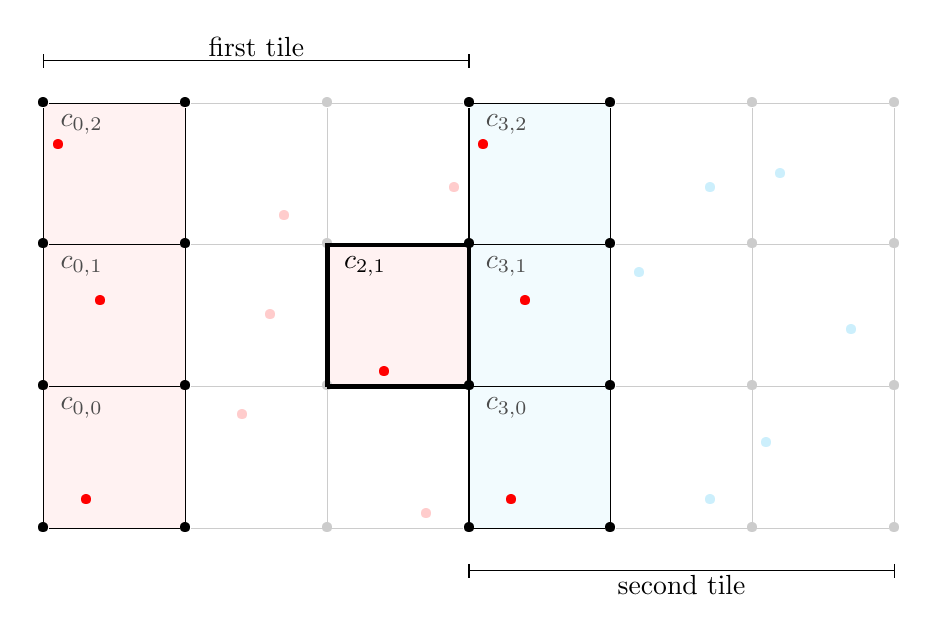
\begin{tikzpicture}[scale=0.9, x=2cm,y=2cm]
    \tikzset{c/.style = {shorten <=-4pt, shorten >=-4pt}}
    \tikzset{smalledge/.style = {-{Latex[length=2mm]},shorten <=-4pt}}
    
    % tile label 1
    \draw (0,3.3) -- (3,3.3);
    \draw (0,3.25) -- (0,3.35);
    \draw (3,3.25) -- (3,3.35);
    \node at (1.5,3.4) {first tile};
    
    % tile label 2
    \draw (3,-0.3) -- (6,-0.3);
    \draw (3,-0.25) -- (3,-0.35);
    \draw (6,-0.25) -- (6,-0.35);
    \node at (4.5,-0.4) {second tile};

    \node (offset) at (3.0,0) {};

    \fill[red!5] (0,0) rectangle (1,3);
    \fill[cyan!5] (3,0) rectangle (4,3);
    \fill[red!5] (2,1) rectangle (3,2);

    \node (x1y1) at (0,0) {\textbullet};
    \node (x2y1) at (1,0) {\textbullet};
    \node[black!20] (x3y1) at (2,0) {\textbullet};
    \node (x4y1) at (3,0) {\textbullet};

    \node (x1y2) at (0,1) {\textbullet};
    \node (x2y2) at (1,1) {\textbullet};
    \node[black!20] (x3y2) at (2,1) {\textbullet};
    \node (x4y2) at (3,1) {\textbullet};

    \node (x1y3) at (0,2) {\textbullet};
    \node (x2y3) at (1,2) {\textbullet};
    \node[black!20] (x3y3) at (2,2) {\textbullet};
    \node (x4y3) at (3,2) {\textbullet};

    \node (x1y4) at (0,3) {\textbullet};
    \node (x2y4) at (1,3) {\textbullet};
    \node[black!20] (x3y4) at (2,3) {\textbullet};
    \node (x4y4) at (3,3) {\textbullet};

    \draw[c] (x1y1) edge node{} (x2y1);
    \draw[c] (x1y2) edge node{} (x2y2);
    \draw[c] (x1y3) edge node{} (x2y3);
    \draw[c] (x1y4) edge node{} (x2y4);
    \draw[c,black!20] (x2y1) edge node{} (x4y1);
    \draw[c,black!20] (x2y2) edge node{} (x4y2);
    \draw[c,black!20] (x2y3) edge node{} (x4y3);
    \draw[c,black!20] (x2y4) edge node{} (x4y4);

    \draw[c] (x1y1) edge node{} (x1y4);
    \draw[c] (x2y1) edge node{} (x2y4);
    \draw[c,black!20] (x3y1) edge node{} (x3y4);
    \draw[c] (x4y1) edge node{} (x4y4);

    \node[red] (s1) at (0.3,0.2) {\textbullet};
    \node[red!20] (s2) at (1.4,0.8) {\textbullet};
    \node[red!20] (s3) at (2.7,0.1) {\textbullet};
    \node[red] (s4) at (0.4,1.6) {\textbullet};
    \node[red!20] (s5) at (1.6,1.5) {\textbullet};
    \node[red] (s6) at (2.4,1.1) {\textbullet};
    \node[red] (s7) at (0.1,2.7) {\textbullet};
    \node[red!20] (s8) at (1.7,2.2) {\textbullet};
    \node[red!20] (s9) at (2.9,2.4) {\textbullet};

    \node (x1y1) at ($(offset) + (0,0)$) {};
    \node (x2y1) at ($(offset) + (1,0)$) {\textbullet};
    \node[black!20] (x3y1) at ($(offset) + (2,0)$) {\textbullet};
    \node[black!20] (x4y1) at ($(offset) + (3,0)$) {\textbullet};

    \node (x1y2) at ($(offset) + (0,1)$) {};
    \node (x2y2) at ($(offset) + (1,1)$) {\textbullet};
    \node[black!20] (x3y2) at ($(offset) + (2,1)$) {\textbullet};
    \node[black!20] (x4y2) at ($(offset) + (3,1)$) {\textbullet};

    \node (x1y3) at ($(offset) + (0,2)$) {};
    \node (x2y3) at ($(offset) + (1,2)$) {\textbullet};
    \node[black!20] (x3y3) at ($(offset) + (2,2)$) {\textbullet};
    \node[black!20] (x4y3) at ($(offset) + (3,2)$) {\textbullet};

    \node (x1y4) at ($(offset) + (0,3)$) {};
    \node (x2y4) at ($(offset) + (1,3)$) {\textbullet};
    \node[black!20] (x3y4) at ($(offset) + (2,3)$) {\textbullet};
    \node[black!20] (x4y4) at ($(offset) + (3,3)$) {\textbullet};

    \draw[c] (x1y1) edge node{} (x2y1);
    \draw[c] (x1y2) edge node{} (x2y2);
    \draw[c] (x1y3) edge node{} (x2y3);
    \draw[c] (x1y4) edge node{} (x2y4);
    \draw[c,black!20] (x2y1) edge node{} (x4y1);
    \draw[c,black!20] (x2y2) edge node{} (x4y2);
    \draw[c,black!20] (x2y3) edge node{} (x4y3);
    \draw[c,black!20] (x2y4) edge node{} (x4y4);

    \draw[c] (x2y1) edge node{} (x2y4);
    \draw[c,black!20] (x3y1) edge node{} (x3y4);
    \draw[c,black!20] (x4y1) edge node{} (x4y4);

    \node[red] (s1) at ($(offset) + (0.3,0.2)$) {\textbullet};
    \node[cyan!20] (s2) at ($(offset) + (1.7,0.2)$) {\textbullet};
    \node[cyan!20] (s3) at ($(offset) + (2.1,0.6)$) {\textbullet};
    \node[red] (s4) at ($(offset) + (0.4,1.6)$) {\textbullet};
    \node[cyan!20] (s5) at ($(offset) + (1.2,1.8)$) {\textbullet};
    \node[cyan!20] (s6) at ($(offset) + (2.7,1.4)$) {\textbullet};
    \node[red] (s7) at ($(offset) + (0.1,2.7)$) {\textbullet};
    \node[cyan!20] (s8) at ($(offset) + (1.7,2.4)$) {\textbullet};
    \node[cyan!20] (s9) at ($(offset) + (2.2,2.5)$) {\textbullet};

    % cell label
    \node[anchor=west] at (2.05,1.85) {$c_{2,1}$};
    \node[black!70,anchor=west] at (0.05,0.85) {$c_{0,0}$};
    \node[black!70,anchor=west] at (0.05,1.85) {$c_{0,1}$};
    \node[black!70,anchor=west] at (0.05,2.85) {$c_{0,2}$};
    \node[black!70,anchor=west] at (3.05,0.85) {$c_{3,0}$};
    \node[black!70,anchor=west] at (3.05,1.85) {$c_{3,1}$};
    \node[black!70,anchor=west] at (3.05,2.85) {$c_{3,2}$};
    \draw[line width=0.6mm] (2,1) -- (3,1) -- (3,2) -- (2,2) -- (2,1);

    \end{tikzpicture}
    \captionof{figure}{Voronoi \gls{noise} seeds that exceed the boundary are sampled from the first set again.}
    \label{img:tikz:noise:seamless:3}
\end{figure}

\noindent
In conclusion, the same set of points that is calculated for the first texture tile needs to be used again for every succeeding tile.

\pagebreak

\noindent
Mathematically, this is solved by using the $modulo$ operation. The dividend is the current cell and the divisor is the period, or how often the \gls{noise} texture is repeated. 

\begin{lstlisting}[language=HLSL, caption=Implementation of a partially seamless 3D Voronoi \gls{noise} algorithm., label=lst:shader:noise:voronoi3d]
    float voronoi(float3 p, float3 period) {
        float3 baseCell = floor(p);
        float dMin = 999;
    
        for(int x = -1; x <= 1; x++) {
            for(int y = -1; y <= 1; y++) {
                for(int z = -1; z <= 1; z++) {
                    float3 cell = baseCell + float3(x, y, z);
                    float3 tiledCell = cell % period;
                    float3 seed = cell + randomSeed(tiledCell);
                    float d = distance(seed, p);
                    if (d < dMin) {
                        dMin = d;
                    }
                }
            }
        }
        
        return dMin;
    }
\end{lstlisting}

\noindent
Interestingly, this does only partially solve the problem. As it turns out, the modulo operation of the \gls{hlsl} treats negative values differently than expected.
Instead of returning the absolute modulo value, it returns the remainder, including negative values.
$$
\begin{array}{l}
    expected: -5 \bmod 3 = 1 \\
    \phantom{ex}actual: -5 \bmod 3 = -2
\end{array}
$$

\noindent
When used this way, the outcome still has visible seams where cell modulo operations has to deal with negative numbers.
The issue is further explained by Ronja \cite{ronja:tilingnoise}.

\begin{figure}[H]
    \includegraphics[width=\linewidth]{noise/voronoi seamless1.png}
    \caption{Partially seamless, tiled 3D \gls{noise} \gls{textureslice}.}
    \label{img:rnd:noise:seamless1}
\end{figure}

\pagebreak

\noindent
The problem is easily fixed, though. Instead of using \gls{hlsl}'s formula, the modulo operation described in the OpenGL documentation \cite{opengl:mod} can be used.
It is defined as follows:
$$
\begin{array}{l}
    mod(x, y) = x - y * floor(x/y)
\end{array}
$$

\noindent
With this implemented, the algorithm needs to be changed only slightly.

\begin{lstlisting}[language=HLSL, caption=Implementation of seamless 3D Voronoi \gls{noise} algorithm., label=lst:shader:noise:voronoi3d]
    #define mod(x,y) (x-y*floor(x/y))

    float voronoi(float3 p, float3 period) {
        float3 baseCell = floor(p);
        float dMin = 999;
    
        for(int x = -1; x <= 1; x++) {
            for(int y = -1; y <= 1; y++) {
                for(int z = -1; z <= 1; z++) {
                    float3 cell = baseCell + float3(x, y, z);
                    float3 tiledCell = mod(cell, period);
                    float3 seed = cell + randomSeed(tiledCell);
                    float d = distance(seed, p);
                    if (d < dMin) {
                        dMin = d;
                    }
                }
            }
        }
        
        return dMin;
    }
\end{lstlisting}

\noindent
And with that, the \gls{noise} texture tiles seamlessly.

\begin{figure}[H]
    \includegraphics[width=\linewidth]{noise/voronoi seamless2.png}
    \caption{Seamlessly tiled 3D \gls{noise} \gls{textureslice}.}
    \label{img:rnd:noise:seamless2}
\end{figure}

\subsection{Compute Shaders}
\label{section:noise:compute}

\subsection{3D Noise Texture Sampling}
\label{section:noise:tex3d}
\clearpage

\printnoidxglossary 
\clearpage
\printbibliography[heading=bibintoc]
\clearpage
\phantomsection
\addcontentsline{toc}{section}{Listings}
\phantomsection
\addcontentsline{toc}{subsection}{Figures}
\listoffigures
\clearpage
\phantomsection
\addcontentsline{toc}{subsection}{Code Listings}
\lstlistoflistings

\end{document}
